\begin{task}
\TT{Wyznacz współczynniki zespolonego szeregu Fouriera dla okresowego sygnału $f(t)$ przedstawionego na rysunku. Narysuj widmo amplitudowe i fazowe sygnału.}{Calculate coefficients of the periodic signal $f(t)$ shown below for the expansion into a complex exponential Fourier series. Draw magnitude and phase spectra.} 

\begin{figure}[H]
\centering
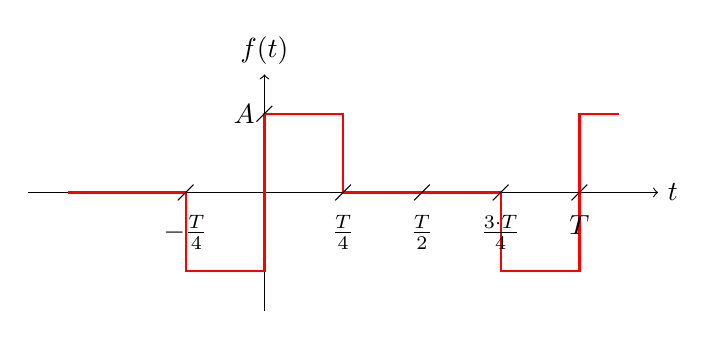
\begin{tikzpicture}
  %\draw (0,0) circle (1in);
  \draw[->] (-3.0,+0.0) -- (+5.0,+0.0) node[right] {$t$};
  \draw[->] (+0.0,-1.5) -- (+0.0,+1.5) node[above] {$f(t)$};
  \draw[-,red, thick] (-2.5,+0.0) -- (-1.0,+0.0) -- (-1.0,-1.0)--(+0.0,-1.0) -- (+0.0,+1.0) -- (+1.0,+1.0) -- (+1.0,+0.0) -- (+3.0,+0.0) -- (+3.0,-1.0) -- (4.0,-1.0) -- (4.0,1.0) -- (4.5,1.0);
  %\draw[-] (-1.0-0.1,-0.1)--(-1.0+0.1,0.1) node[midway, below, outer sep=10pt,align=center] {$-\frac{T}{2}$};
  \draw[-] (-1.0-0.1,-0.1)--(-1.0+0.1,0.1) node[midway, below, outer sep=5pt,align=center] {$-\frac{T}{4}$};
  \draw[-] (+1.0-0.1,-0.1)--(+1.0+0.1,0.1) node[midway, below, outer sep=5pt] {$\frac{T}{4}$};
  \draw[-] (+2.0-0.1,-0.1)--(+2.0+0.1,0.1) node[midway, below, outer sep=5pt] {$\frac{T}{2}$};
  \draw[-] (+3.0-0.1,-0.1)--(+3.0+0.1,0.1) node[midway, below, outer sep=5pt] {$\frac{3\cdot T}{4}$};
  \draw[-] (+4.0-0.1,-0.1)--(+4.0+0.1,0.1) node[midway, below, outer sep=5pt] {$T$};
  \draw[-] (-0.1,1.0-0.1)--(+0.1,1.0+0.1) node[midway, left] {$A$};
\end{tikzpicture}
\end{figure}

\TT{W pierwszej kolejności należy opisać sygnał za pomocą wzoru.}{Periodic signal $f(t)$, as a piecewise linear function, is given by:}

\begin{equation}
   f(x)=\begin{cases}-A & t \in \left (  -\frac{T}{4}+k \cdot T; 0+k \cdot T \right ) \\A & t \in \left (  0+k \cdot T; \frac{T}{4}+k \cdot T \right ) \\0 & t \in \left ( \frac{T}{4}+k \cdot T; \frac{3\cdot T}{4} +k \cdot T\right )\end{cases} \wedge k \in \TT{C}{Z}
\end{equation}

\TT{Współczynnik $F_0$ wyznaczamy ze wzoru:}{The $F_0$ coefficient is defined as:}

\begin{equation}
F_0=\frac{1}{T}\int_{T}f(t) \cdot dt
\end{equation}

\TT{Podstawiamy do wzoru wzór naszej funkcji w pierwszym okresie $k=0$}{For the period $t \in (-\frac{T}{4}; \frac{3 \cdot T}{4})$, i.e. $k=0$, we get:}

\begin{equation}
\begin{aligned}
F_0 &=\frac{1}{T}\int_{T}f(t) \cdot dt =\\
&=\frac{1}{T} \left( \int_{-\frac{T}{4}}^{0} -A \cdot dt + 
\int_{0}^{\frac{T}{4}} A \cdot dt +
\int_{\frac{T}{4}}^{\frac{3\cdot T}{4}} 0 \cdot dt \right ) = \\
&=\frac{1}{T} \left( \int_{-\frac{T}{4}}^{0} -A \cdot dt + 
\int_{0}^{\frac{T}{4}} A \cdot dt + 0 \right ) = \\
&=\frac{1}{T} \left( -A \cdot \int_{-\frac{T}{4}}^{0} dt + 
A \cdot \int_{0}^{\frac{T}{4}} dt + 0 \right ) = \\
&=\frac{1}{T} \left( -A \cdot \left. t \right|_{-\frac{T}{4}}^{0} + 
A \cdot \left. t \right|_{0}^{\frac{T}{4}}\right ) = \\
&=\frac{1}{T} \left( -A \cdot \left( 0 - \left(-\frac{T}{4}\right) \right) + 
A \cdot \left( \frac{T}{4} - 0 \right)\right ) = \\
&=\frac{1}{T} \left( -A \cdot \frac{T}{4} + 
A \cdot \frac{T}{4}\right ) = \\
&=\frac{1}{T} \left( 0 \right ) = \\
&=0
\end{aligned}
\end{equation}

\TT{Wartość współczynnika $F_0$ wynosi $0$.}{The $F_0$ coefficient equals $0$.}


\TT{Współczynniki $F_k$ wyznaczamy ze wzoru:}{The $F_k$ coefficients are defined as:}

\begin{equation}
F_k=\frac{1}{T}\int_{T}f(t) \cdot e^{-\jmath \cdot  k \cdot \frac{2\pi}{T} \cdot t} \cdot dt
\end{equation}

\TT{Podstawiamy do wzoru wzór naszej funkcji w pierwszym okresie $k=0$}{For the period $t \in (-\frac{T}{4}; \frac{3 \cdot T}{4})$, i.e. $k=0$, we get:}

\begin{align*}
F_k&=\frac{1}{T}\int_{T}f(t) \cdot e^{-\jmath \cdot k \cdot \frac{2\pi}{T} \cdot t} \cdot dt=\\
&=\frac{1}{T}\left(\int_{-\frac{T}{4}}^{0} -A \cdot e^{-\jmath \cdot k \cdot \frac{2\pi}{T} \cdot t} \cdot dt 
+ \int_{0}^{\frac{T}{4}} A \cdot e^{-\jmath \cdot k \cdot \frac{2\pi}{T} \cdot t} \cdot dt
+ \int_{\frac{T}{4}}^{\frac{3\cdot T}{4}} 0 \cdot e^{-\jmath \cdot k \cdot \frac{2\pi}{T} \cdot t} \cdot dt \right)=\\
&=\frac{1}{T}\left(-A \cdot \int_{-\frac{T}{4}}^{0} e^{-\jmath \cdot k \cdot \frac{2\pi}{T} \cdot t} \cdot dt 
+ A \cdot \int_{0}^{\frac{T}{4}} e^{-\jmath \cdot k \cdot \frac{2\pi}{T} \cdot t} \cdot dt
+ \int_{\frac{T}{4}}^{\frac{3\cdot T}{4}} 0 \cdot dt \right)=\\
&=\begin{Bmatrix*}[l]
z&=-\jmath \cdot k \cdot \frac{2\pi}{T} \cdot t \\
dz&=-\jmath \cdot k \cdot \frac{2\pi}{T} \cdot dt \\
dt&=\frac{dz}{-\jmath \cdot k \cdot \frac{2\pi}{T}}
\end{Bmatrix*} =\\
&=\frac{1}{T}\left(-A \cdot \int_{-\frac{T}{4}}^{0} e^{ z } \cdot \frac{dz}{-\jmath \cdot k \cdot \frac{2\pi}{T}} 
+ A \cdot \int_{0}^{\frac{T}{4}} e^{ z } \cdot \frac{dz}{-\jmath 
 \cdot k \cdot \frac{2\pi}{T}}
+ 0 \right)=\\
&=\frac{1}{T}\left(-\frac{A}{-\jmath \cdot k \cdot \frac{2\pi}{T}} \cdot \int_{-\frac{T}{4}}^{0} e^{ z } \cdot dz 
+ \frac{A}{-\jmath \cdot k \cdot \frac{2\pi}{T}} \cdot \int_{0}^{\frac{T}{4}} e^{ z } \cdot dz\right)=\\
&=\frac{1}{T} \cdot \frac{A}{\jmath \cdot k \cdot \frac{2\pi}{T}} \cdot \left( \left. e^{ z } \right|_{-\frac{T}{4}}^{0}
- \left. e^{ z }\right|_{0}^{\frac{T}{4}} \right)=\\
&=\frac{A}{\jmath \cdot k \cdot 2\pi} \cdot \left( \left. e^{ -\jmath \cdot k \cdot \frac{2\pi}{T} \cdot t  } \right|_{-\frac{T}{4}}^{0}
- \left. e^{ -\jmath \cdot k \cdot \frac{2\pi}{T} \cdot t  }\right|_{0}^{\frac{T}{4}} \right)=\\
&=\frac{A}{\jmath \cdot k \cdot 2\pi} \cdot \left(\left( e^{ -\jmath \cdot k \cdot \frac{2\pi}{T} \cdot 0  } - e^{ \jmath \cdot  k \cdot \frac{2\pi}{T} \cdot \frac{T}{4}  } \right)
- \left( e^{ -\jmath \cdot k \cdot \frac{2\pi}{T} \cdot \frac{T}{4}  } - e^{ -\jmath \cdot k \cdot \frac{2\pi}{T} \cdot 0  }\right) \right)=\\
&=\frac{A}{\jmath \cdot k \cdot 2\pi} \cdot \left(\left( e^{ 0 } - e^{ \jmath \cdot k \cdot \frac{2\pi}{4} } \right)
- \left( e^{ -\jmath \cdot k \cdot \frac{2\pi}{4} } - e^{ 0 }\right) \right)=\\
&=\frac{A}{\jmath \cdot k \cdot 2\pi} \cdot \left(\left( 1 - e^{ \jmath \cdot k \cdot \frac{\pi}{2} } \right)
- \left( e^{-\jmath \cdot k \cdot \frac{\pi}{2} } - 1\right) \right)=\\
&=\frac{A}{\jmath \cdot k \cdot 2\pi} \cdot \left(1 - e^{ \jmath \cdot k \cdot \frac{\pi}{2} } - e^{-\jmath \cdot k \cdot \frac{\pi}{2} } + 1 \right)=\\
&=\frac{A}{\jmath \cdot k \cdot 2\pi} \cdot \left(2 - \left(e^{ \jmath \cdot k \cdot \frac{\pi}{2} } + e^{-\jmath \cdot k \cdot \frac{\pi}{2} } \right) \right)=\\
&=\frac{A}{\jmath \cdot k \cdot 2\pi} \cdot 2 \cdot \left(1 - \frac{e^{ \jmath \cdot k \cdot \frac{\pi}{2} } + e^{-\jmath \cdot k \cdot \frac{\pi}{2} } }{2} \right)=\\
&=\frac{A}{\jmath \cdot k \cdot \pi} \cdot \left(1 - \frac{e^{ \jmath \cdot k \cdot \frac{\pi}{2} } + e^{-\jmath \cdot k \cdot \frac{\pi}{2} } }{2} \right)=\\
&=\begin{Bmatrix*}[l]
cos(x)&=\frac{e^{\jmath \cdot x}+e^{-\jmath \cdot x}}{2}
\end{Bmatrix*}=\\
&=\frac{A}{\jmath \cdot k \cdot \pi} \cdot \left(1 - cos\left( k \cdot \frac{\pi}{2} \right) \right)=\\
&=-\jmath \cdot \frac{A}{k \cdot \pi} \cdot \left(1 - cos\left( k \cdot \frac{\pi}{2} \right) \right)=\\
&=\jmath \cdot \frac{A}{k \cdot \pi} \cdot \left(cos\left( k \cdot \frac{\pi}{2} \right) - 1\right)
\end{align*}

\TT{Wartość współczynnika $F_k$ wynosi $\jmath \cdot \frac{A}{k \cdot \pi} \cdot \left(cos\left( k \cdot \frac{\pi}{2} \right) - 1\right)$.}{The $F_k$ coefficients equal to $\jmath \cdot \frac{A}{k \cdot \pi} \cdot \left(cos\left( k \cdot \frac{\pi}{2} \right) - 1\right)$.}

\TT{Ostatecznie współczynniki zespolonego szeregu Fouriera dla funkcji przedstawionej na rysunku przyjmują wartości.}{To sum up, coefficients for the expansion into a complex exponential Fourier series are given by:}

\begin{equation}
\begin{aligned}
F_0&=0\\
F_k&=\jmath \cdot \frac{A}{k \cdot \pi} \cdot \left(cos\left( k \cdot \frac{\pi}{2} \right) - 1\right)\\
\end{aligned}
\end{equation}

\TT{Podstawiając to wzoru aproksymacyjnego funkcje $f(t)$ możemy wyrazić jako}{Hence, the signal $f(t)$ may be expressed as the sum of the harmonic series}

\begin{equation}
\begin{aligned}
f(t) &= \sum_{k=-\infty}^{\infty} F_k \cdot e^{k \cdot \frac{2\pi}{T} \cdot t}\\
f(t) &= \sum_{\begin{smallmatrix}k=-\infty \\ k \neq 0 \end{smallmatrix}}^{\infty} \left[\jmath \cdot \frac{A}{k \cdot \pi} \cdot \left(cos\left( k \cdot \frac{\pi}{2} \right) - 1\right)\right] \cdot e^{\jmath \cdot k \cdot \frac{2\pi}{T} \cdot t}
\end{aligned}
\end{equation}

\TT{Możemy wyznaczyć kilka wartości współczynników $F_k$}{The first several coefficients are equal to:}

\begin{table}[H]
\centering  
\begin{tabular}{|c|c|c|c|c|c|c|c|c|c|c|c|c|c|}
  \hline 
  $k$ & $-6$ & $-5$ & $-4$ & $-3$ & $-2$ & $-1$ & $0$ & $1$ & $2$ & $3$ & $4$ & $5$ & $6$\\ 
  \hline 
  $F_k$ & $\jmath \cdot \frac{A}{3\pi}$ & $\jmath \cdot \frac{A}{5\pi}$ & $0$ & $\jmath \cdot \frac{A}{3\pi}$ & $\jmath \cdot \frac{A}{\pi}$ & $\jmath \cdot \frac{A}{\pi}$ & $0$ & $-\jmath \cdot \frac{A}{\pi}$ & $-\jmath \cdot \frac{A}{\pi}$ & $-\jmath \cdot \frac{A}{3\pi}$ & $0$ & $-\jmath \cdot \frac{A}{5\pi}$ & $-\jmath \cdot \frac{A}{3\pi}$\\
  \hline 
  $\left|F_k\right|$ & $\frac{A}{3\pi}$ & $\frac{A}{5\pi}$ & $0$ & $\frac{A}{3\pi}$ & $\frac{A}{\pi}$ & $\frac{A}{\pi}$ & $0$ & $\frac{A}{\pi}$ & $\frac{A}{\pi}$ & $\frac{A}{3\pi}$ & $0$ & $\frac{A}{5\pi}$ & $\frac{A}{3\pi}$\\
  \hline
  $Arg\left\{ F_k \right\}$ & $\frac{\pi}{2}$ & $\frac{\pi}{2}$ & $0$ & $\frac{\pi}{2}$ & $\frac{\pi}{2}$ & $\frac{\pi}{2}$ & $0$ & $-\frac{\pi}{2}$ & $-\frac{\pi}{2}$ & $-\frac{\pi}{2}$ & $0$ & $-\frac{\pi}{2}$ & $-\frac{\pi}{2}$\\
  \hline 
  
\end{tabular} 
\end{table}

\TT{Na podstawie wyznaczonych współczynników $F_k$ możemy narysować widmo amplitudowe $\left|F_k\right|$ sygnału $f(t)$.}{Based on coefficents $F_k$ we can plot magnitude spectrum $\left|F_k\right|$ of the $f(t)$ signal.}

\begin{figure}[H]
    \centering
    \begin{tikzpicture}
    
    \tikzmath{
        function mFk(\k,\A) {
            if(\k==0) then
            {
                return 0;
            }
            else
            {
                return abs(\A/(\k*3.141592)*(sqrt((cos(\k*90)-1.0)^2)));       
            };
        };
    }
    
    %\draw (0,0) circle (1in);
    \draw[->] (-6.0,+0.0) -- (+6.0,+0.0) node[right] {$k$};
    \draw[->] (+0.0,-0.0) -- (+0.0,+2.5) node[above] {$\left|F_k\right|$};
    \draw[-] (-0.1,2.0-0.1)--(+0.1,2.0+0.1) node[midway, left] {$\frac{A}{\pi}$};
    
    \foreach \k in {-8,-7,...,8 }{
        \pgfmathsetmacro{\x}{\k/1.5};
        \draw[-] ({\x-0.1},-0.1)--({\x+0.1},0.1) node[midway, below, outer sep=5pt] {${\k}$};    
    };
    
    \foreach \k in {-8,-7,...,8 }{
        \pgfmathsetmacro{\x}{\k/1.5};
        \pgfmathsetmacro{\y}{mFk(\k,4)*3.141592/2.0};
        \node[circle,red,fill=red,scale=0.5] (\x\y) at (\x,\y) {};
        \draw[-, red] (\x,0) -- (\x,\y);
    };
    
    \end{tikzpicture}
\end{figure}

\TT{Widmo aplitudowe sygnału rzeczywistego jest zawsze parzyste.}{The magnitude spectrum of a \underline{real signal} is an even-symmetric function of $k$.}

\TT{Podobnie n podstawie wyznaczonych współczynników $F_k$ możemy narysować widmo fazowe $\mathtt{arg}\left\{F_k\right\}$ sygnału $f(t)$.}{Based on coefficents $F_k$ we can plot phase spectrum $\mathtt{arg}\left\{F_k\right\}$ of the $f(t)$ signal.}

\begin{figure}[H]
    \centering
    \begin{tikzpicture}
    
    \tikzmath{
        function aFk(\k,\A) {
            if(mod(\k,4)==0) then
            {
                return 0;
            }
            else
            {
                if(\k<0) then 
                {
                    return 3.141592/2;
                }
                else
                {
                    return -3.141592/2;                    
                };
            };
        };
    }
    
    %\draw (0,0) circle (1in);
    \draw[->] (-6.0,+0.0) -- (+6.0,+0.0) node[right] {$k$};
    \draw[->] (+0.0,-2.5) -- (+0.0,+2.5) node[above] {$\mathtt{arg}\left\{F_k\right\}$};
    \draw[-] (-0.1,2.0-0.1)--(+0.1,2.0+0.1) node[midway, left] {$\pi$};
    \draw[-] (-0.1,-2.0-0.1)--(+0.1,-2.0+0.1) node[midway, left] {$-\pi$};
    \draw[-] (-0.1,1.0-0.1)--(+0.1,1.0+0.1) node[midway, left] {$\frac{\pi}{2}$};
    \draw[-] (-0.1,-1.0-0.1)--(+0.1,-1.0+0.1) node[midway, left] {$-\frac{\pi}{2}$};
    
    \foreach \k in {-8,-7,...,8 }{
        \pgfmathsetmacro{\x}{\k/1.5};
        \draw[-] ({\x-0.1},-0.1)--({\x+0.1},0.1) node[midway, below, outer sep=5pt] {${\k}$};    
    };
    
    \foreach \k in {-8,-7,...,8 }{
        \pgfmathsetmacro{\x}{\k/1.5};
        \pgfmathsetmacro{\y}{aFk(\k,4)*2.0/3.141592};
        \node[circle,red,fill=red,scale=0.5] (\x\y) at (\x,\y) {};
        \draw[-, red] (\x,0) -- (\x,\y);
    };
    
    \end{tikzpicture}
\end{figure}

\TT{Widmo fazowe sygnału rzeczywistego jest zawsze nieparzyste.}{The phase spectrum of a \underline{real signal} is an odd-symmetric function of $k$.}

\TT{W przypadku sumowania od $k_{min}=-1$ do $k_{max}=1$ otrzymujemy:}{A partial approximation of the $f(t)$ signal from $k_{min}=-1$ to $k_{max}=1$ results in:}

\begin{figure}[H]
  \centering
  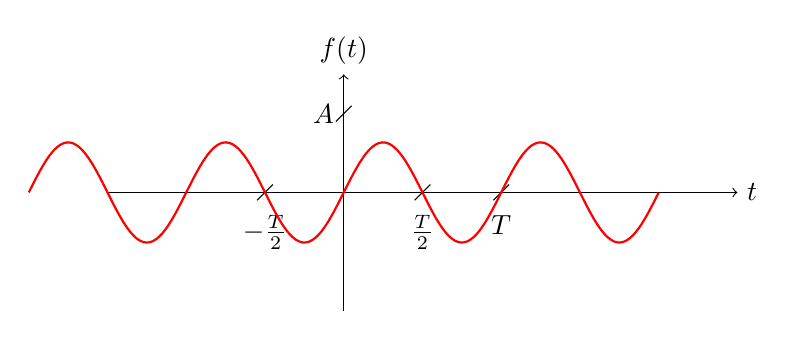
\begin{tikzpicture}
  %\draw (0,0) circle (1in);
  \draw[->] (-3.0,+0.0) -- (+5.0,+0.0) node[right] {$t$};
  \draw[->] (+0.0,-1.5) -- (+0.0,+1.5) node[above] {$f(t)$};
  %\draw[-,red, thick] (-2.5,+0.0) -- (+0.0,+0.0);
  %\draw[-] (-1.0-0.1,-0.1)--(-1.0+0.1,0.1) node[midway, below, outer sep=10pt,align=center] {$-\frac{T}{2}$};
  \draw[-] (-1.0-0.1,-0.1)--(-1.0+0.1,0.1) node[midway, below, outer sep=5pt,align=center] {$-\frac{T}{2}$};
  \draw[-] (+1.0-0.1,-0.1)--(+1.0+0.1,0.1) node[midway, below, outer sep=5pt] {$\frac{T}{2}$};
  \draw[-] (+2.0-0.1,-0.1)--(+2.0+0.1,0.1) node[midway, below, outer sep=5pt] {$T$};
  \draw[-] (-0.1,1.0-0.1)--(+0.1,1.0+0.1) node[midway, left] {$A$};
  
  \draw[scale=1.0,domain=-4:4.0,samples=100,smooth,variable=\x,red,thick] plot ({\x},{0.0+2.0/3.141592*sin(\x*180.0/3.141592*1*3.141592/1.0)});
  \end{tikzpicture}
\end{figure}

\TT{W przypadku sumowania od $k_{min}=-2$ do $k_{max}=2$ otrzymujemy:}{A partial approximation of the $f(t)$ signal from $k_{min}=-2$ to $k_{max}=2$ results in:}

\begin{figure}[H]
  \centering
  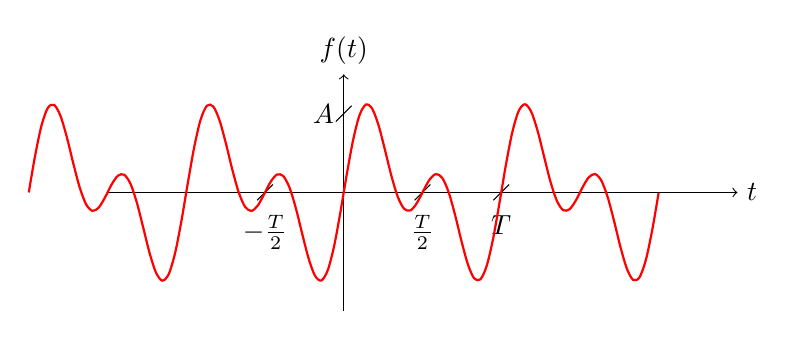
\begin{tikzpicture}
  %\draw (0,0) circle (1in);
  \draw[->] (-3.0,+0.0) -- (+5.0,+0.0) node[right] {$t$};
  \draw[->] (+0.0,-1.5) -- (+0.0,+1.5) node[above] {$f(t)$};
  %\draw[-,red, thick] (-2.5,+0.0) -- (+0.0,+0.0);
  %\draw[-] (-1.0-0.1,-0.1)--(-1.0+0.1,0.1) node[midway, below, outer sep=10pt,align=center] {$-\frac{T}{2}$};
  \draw[-] (-1.0-0.1,-0.1)--(-1.0+0.1,0.1) node[midway, below, outer sep=5pt,align=center] {$-\frac{T}{2}$};
  \draw[-] (+1.0-0.1,-0.1)--(+1.0+0.1,0.1) node[midway, below, outer sep=5pt] {$\frac{T}{2}$};
  \draw[-] (+2.0-0.1,-0.1)--(+2.0+0.1,0.1) node[midway, below, outer sep=5pt] {$T$};
  \draw[-] (-0.1,1.0-0.1)--(+0.1,1.0+0.1) node[midway, left] {$A$};
  
  \draw[scale=1.0,domain=-4:4.0,samples=100,smooth,variable=\x,red,thick] plot ({\x},{0.0+2.0/3.141592*sin(\x*180.0/3.141592*1*3.141592/1.0)+2.0/(3.141592)*sin(\x*180.0/3.141592*2*3.141592/1.0)});
  \end{tikzpicture}
\end{figure}

\TT{W przypadku sumowania od $k_{min}=-3$ do $k_{max}=3$ otrzymujemy:}{A partial approximation of the $f(t)$ signal from $k_{min}=-3$ to $k_{max}=3$ results in:}

\begin{figure}[H]
  \centering
  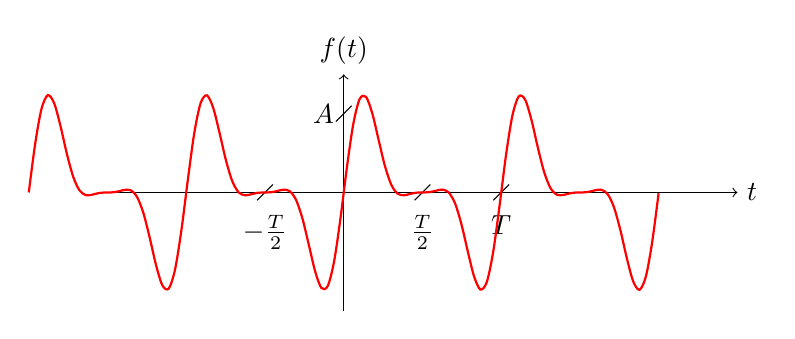
\begin{tikzpicture}
  %\draw (0,0) circle (1in);
  \draw[->] (-3.0,+0.0) -- (+5.0,+0.0) node[right] {$t$};
  \draw[->] (+0.0,-1.5) -- (+0.0,+1.5) node[above] {$f(t)$};
  %\draw[-,red, thick] (-2.5,+0.0) -- (+0.0,+0.0);
  %\draw[-] (-1.0-0.1,-0.1)--(-1.0+0.1,0.1) node[midway, below, outer sep=10pt,align=center] {$-\frac{T}{2}$};
  \draw[-] (-1.0-0.1,-0.1)--(-1.0+0.1,0.1) node[midway, below, outer sep=5pt,align=center] {$-\frac{T}{2}$};
  \draw[-] (+1.0-0.1,-0.1)--(+1.0+0.1,0.1) node[midway, below, outer sep=5pt] {$\frac{T}{2}$};
  \draw[-] (+2.0-0.1,-0.1)--(+2.0+0.1,0.1) node[midway, below, outer sep=5pt] {$T$};
  \draw[-] (-0.1,1.0-0.1)--(+0.1,1.0+0.1) node[midway, left] {$A$};
  
  \draw[scale=1.0,domain=-4:4.0,samples=100,smooth,variable=\x,red,thick] plot ({\x},{0.0+2.0/3.141592*sin(\x*180.0/3.141592*1*3.141592/1.0)+2.0/(1*3.141592)*sin(\x*180.0/3.141592*2*3.141592/1.0)+2.0/(3*3.141592)*sin(\x*180.0/3.141592*3*3.141592/1.0)});
  \end{tikzpicture}
\end{figure}

\TT{W przypadku sumowania od $k_{min}=-5$ do $k_{max}=5$ otrzymujemy:}{A partial approximation of the $f(t)$ signal from $k_{min}=-5$ to $k_{max}=5$ results in:}

\begin{figure}[H]
  \centering
  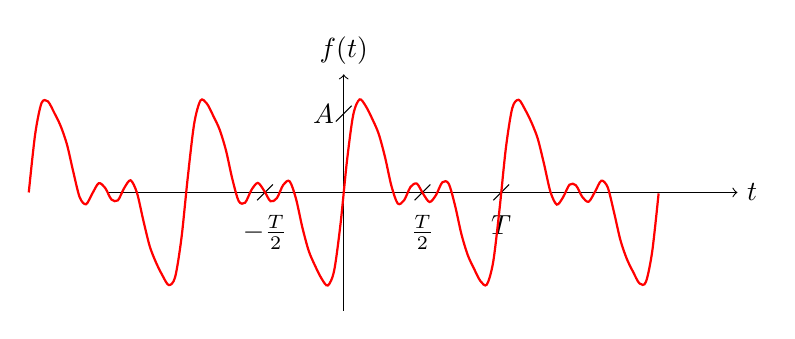
\begin{tikzpicture}
  %\draw (0,0) circle (1in);
  \draw[->] (-3.0,+0.0) -- (+5.0,+0.0) node[right] {$t$};
  \draw[->] (+0.0,-1.5) -- (+0.0,+1.5) node[above] {$f(t)$};
  %\draw[-,red, thick] (-2.5,+0.0) -- (+0.0,+0.0);
  %\draw[-] (-1.0-0.1,-0.1)--(-1.0+0.1,0.1) node[midway, below, outer sep=10pt,align=center] {$-\frac{T}{2}$};
  \draw[-] (-1.0-0.1,-0.1)--(-1.0+0.1,0.1) node[midway, below, outer sep=5pt,align=center] {$-\frac{T}{2}$};
  \draw[-] (+1.0-0.1,-0.1)--(+1.0+0.1,0.1) node[midway, below, outer sep=5pt] {$\frac{T}{2}$};
  \draw[-] (+2.0-0.1,-0.1)--(+2.0+0.1,0.1) node[midway, below, outer sep=5pt] {$T$};
  \draw[-] (-0.1,1.0-0.1)--(+0.1,1.0+0.1) node[midway, left] {$A$};
  
  \draw[scale=1.0,domain=-4:4.0,samples=100,smooth,variable=\x,red,thick] plot ({\x},{0.0+2.0/3.141592*sin(\x*180.0/3.141592*1*3.141592/1.0)+2.0/(1*3.141592)*sin(\x*180.0/3.141592*2*3.141592/1.0)+2.0/(3*3.141592)*sin(\x*180.0/3.141592*3*3.141592/1.0)+2.0/(5*3.141592)*sin(\x*180.0/3.141592*5*3.141592/1.0)});
  \end{tikzpicture}
\end{figure}

\TT{W przypadku sumowania od $k_{min}=-6$ do $k_{max}=6$ otrzymujemy:}{A partial approximation of the $f(t)$ signal from $k_{min}=-6$ to $k_{max}=6$ results in:}

\begin{figure}[H]
  \centering
  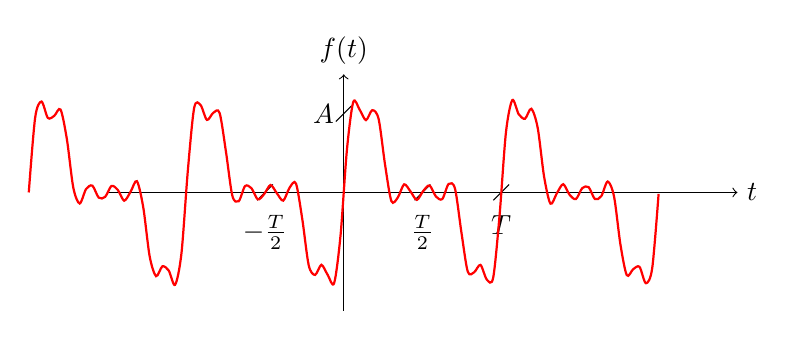
\begin{tikzpicture}
  %\draw (0,0) circle (1in);
  \draw[->] (-3.0,+0.0) -- (+5.0,+0.0) node[right] {$t$};
  \draw[->] (+0.0,-1.5) -- (+0.0,+1.5) node[above] {$f(t)$};
  %\draw[-,red, thick] (-2.5,+0.0) -- (+0.0,+0.0);
  %\draw[-] (-1.0-0.1,-0.1)--(-1.0+0.1,0.1) node[midway, below, outer sep=10pt,align=center] {$-\frac{T}{2}$};
  \draw[-] (-1.0-0.1,-0.1)--(-1.0+0.1,0.1) node[midway, below, outer sep=5pt,align=center] {$-\frac{T}{2}$};
  \draw[-] (+1.0-0.1,-0.1)--(+1.0+0.1,0.1) node[midway, below, outer sep=5pt] {$\frac{T}{2}$};
  \draw[-] (+2.0-0.1,-0.1)--(+2.0+0.1,0.1) node[midway, below, outer sep=5pt] {$T$};
  \draw[-] (-0.1,1.0-0.1)--(+0.1,1.0+0.1) node[midway, left] {$A$};
  
  \draw[scale=1.0,domain=-4:4.0,samples=100,smooth,variable=\x,red,thick] plot ({\x},{0.0+2.0/3.141592*sin(\x*180.0/3.141592*1*3.141592/1.0)+2.0/(1*3.141592)*sin(\x*180.0/3.141592*2*3.141592/1.0)+2.0/(3*3.141592)*sin(\x*180.0/3.141592*3*3.141592/1.0)+2.0/(5*3.141592)*sin(\x*180.0/3.141592*5*3.141592/1.0)+2.0/(3*3.141592)*sin(\x*180.0/3.141592*6*3.141592/1.0)});
  \end{tikzpicture}
\end{figure}

\TT{W przypadku sumowania od $k_{min}=-11$ do $k_{max}=11$ otrzymujemy:}{A partial approximation of the $f(t)$ signal from $k_{min}=-11$ to $k_{max}=11$ results in:} 

\begin{figure}[H]
  \centering
  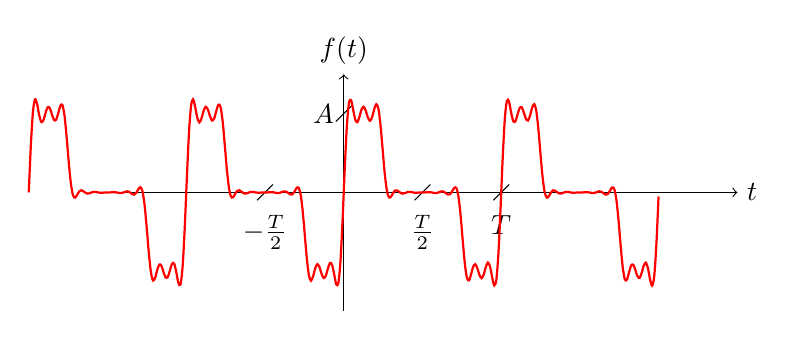
\begin{tikzpicture}
  %\draw (0,0) circle (1in);
  \draw[->] (-3.0,+0.0) -- (+5.0,+0.0) node[right] {$t$};
  \draw[->] (+0.0,-1.5) -- (+0.0,+1.5) node[above] {$f(t)$};
  %\draw[-,red, thick] (-2.5,+0.0) -- (+0.0,+0.0);
  %\draw[-] (-1.0-0.1,-0.1)--(-1.0+0.1,0.1) node[midway, below, outer sep=10pt,align=center] {$-\frac{T}{2}$};
  \draw[-] (-1.0-0.1,-0.1)--(-1.0+0.1,0.1) node[midway, below, outer sep=5pt,align=center] {$-\frac{T}{2}$};
  \draw[-] (+1.0-0.1,-0.1)--(+1.0+0.1,0.1) node[midway, below, outer sep=5pt] {$\frac{T}{2}$};
  \draw[-] (+2.0-0.1,-0.1)--(+2.0+0.1,0.1) node[midway, below, outer sep=5pt] {$T$};
  \draw[-] (-0.1,1.0-0.1)--(+0.1,1.0+0.1) node[midway, left] {$A$};
  
  \draw[scale=1.0,domain=-4:4.0,samples=300,smooth,variable=\x,red,thick] plot ({\x},{0.0+2.0/3.141592*sin(\x*180.0/3.141592*1*3.141592/1.0)+2.0/(1*3.141592)*sin(\x*180.0/3.141592*2*3.141592/1.0)+2.0/(3*3.141592)*sin(\x*180.0/3.141592*3*3.141592/1.0)+2.0/(5*3.141592)*sin(\x*180.0/3.141592*5*3.141592/1.0)+2.0/(3*3.141592)*sin(\x*180.0/3.141592*6*3.141592/1.0)+2.0/(7*3.141592)*sin(\x*180.0/3.141592*7*3.141592/1.0)+2.0/(9*3.141592)*sin(\x*180.0/3.141592*9*3.141592/1.0)+2.0/(5*3.141592)*sin(\x*180.0/3.141592*10*3.141592/1.0)+2.0/(11*3.141592)*sin(\x*180.0/3.141592*11*3.141592/1.0)});
  \end{tikzpicture}
\end{figure}

\TT{W przypadku sumowania od $k_{min}=-21$ do $k_{max}=21$ otrzymujemy:}{A partial approximation of the $f(t)$ signal from $k_{min}=-21$ to $k_{max}=21$ results in:}

\begin{figure}[H]
  \centering
  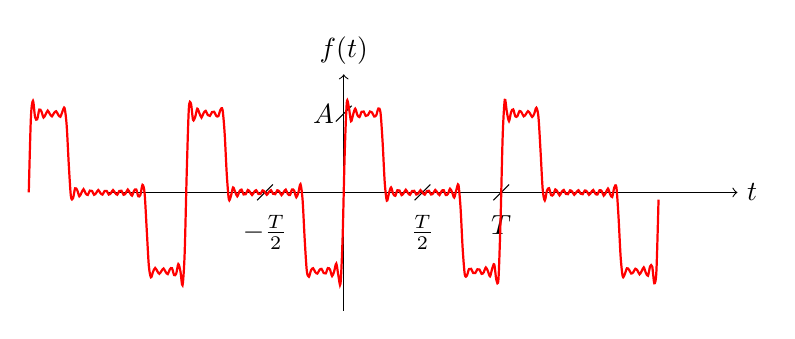
\begin{tikzpicture}
  %\draw (0,0) circle (1in);
  \draw[->] (-3.0,+0.0) -- (+5.0,+0.0) node[right] {$t$};
  \draw[->] (+0.0,-1.5) -- (+0.0,+1.5) node[above] {$f(t)$};
  %\draw[-,red, thick] (-2.5,+0.0) -- (+0.0,+0.0);
  %\draw[-] (-1.0-0.1,-0.1)--(-1.0+0.1,0.1) node[midway, below, outer sep=10pt,align=center] {$-\frac{T}{2}$};
  \draw[-] (-1.0-0.1,-0.1)--(-1.0+0.1,0.1) node[midway, below, outer sep=5pt,align=center] {$-\frac{T}{2}$};
  \draw[-] (+1.0-0.1,-0.1)--(+1.0+0.1,0.1) node[midway, below, outer sep=5pt] {$\frac{T}{2}$};
  \draw[-] (+2.0-0.1,-0.1)--(+2.0+0.1,0.1) node[midway, below, outer sep=5pt] {$T$};
  \draw[-] (-0.1,1.0-0.1)--(+0.1,1.0+0.1) node[midway, left] {$A$};
  
  \draw[scale=1.0,domain=-4:4.0,samples=300,smooth,variable=\x,red,thick] plot ({\x},{0.0+2.0/3.141592*sin(\x*180.0/3.141592*1*3.141592/1.0)+2.0/(1*3.141592)*sin(\x*180.0/3.141592*2*3.141592/1.0)+2.0/(3*3.141592)*sin(\x*180.0/3.141592*3*3.141592/1.0)+2.0/(5*3.141592)*sin(\x*180.0/3.141592*5*3.141592/1.0)+2.0/(3*3.141592)*sin(\x*180.0/3.141592*6*3.141592/1.0)+2.0/(7*3.141592)*sin(\x*180.0/3.141592*7*3.141592/1.0)+2.0/(9*3.141592)*sin(\x*180.0/3.141592*9*3.141592/1.0)+2.0/(5*3.141592)*sin(\x*180.0/3.141592*10*3.141592/1.0)+2.0/(11*3.141592)*sin(\x*180.0/3.141592*11*3.141592/1.0)+2.0/(13*3.141592)*sin(\x*180.0/3.141592*13*3.141592/1.0)+2.0/(7*3.141592)*sin(\x*180.0/3.141592*14*3.141592/1.0)+2.0/(15*3.141592)*sin(\x*180.0/3.141592*15*3.141592/1.0)+2.0/(17*3.141592)*sin(\x*180.0/3.141592*17*3.141592/1.0)+2.0/(9*3.141592)*sin(\x*180.0/3.141592*18*3.141592/1.0)+2.0/(19*3.141592)*sin(\x*180.0/3.141592*19*3.141592/1.0)+2.0/(21*3.141592)*sin(\x*180.0/3.141592*21*3.141592/1.0)});
  \end{tikzpicture}
\end{figure}

\TT{W granicy sumowania od $k_{min}=-\infty$ do $k_{max}=\infty$ otrzymujemy oryginalny sygnał.}{Approximation of the $f(t)$ signal for from $k_{min}=-\infty$ to $k_{max}=\infty$ results in oryginal signal.}

\end{task}